\documentclass[spanish,authorshippage=ltd,pagelimitmode=flex,noloa,nolol]{thesis}[2015/07/11 v1.0.1]

%\documentclass[spanish,noloa,nolol,pagelimitmode=flex,authorshippage=ltd]{thesis} [2015/07/11 v1.0.1]

	% custom commands %
	
\newcommand{\uci}{Universidad de las Ciencias Inform�ticas }
\newcommand{\fac}{Facultad 4 }
\newcommand{\cdis}{Sistema de Gesti�n para el Proceso de Comisi�n Disciplinaria en la Facultad 4 de la Universidad de las Ciencias Inform�ticas}
\newcommand{\stripe}{\rowcolor[HTML]{EDEBF1}}
\newcommand{\theader}{\rowcolor[HTML]{CBCEFB}}
\newcommand{\authorC}{Carlos Enrique Pi�eiro C�rdenas}
\newcommand{\authorA}{�ngel Luis Fumero S�nchez}
\newcommand{\tutorY}{Yordankis Matos L�pez}
\newcommand{\userY}{Yadira Ram�rez Rodr�guez}

% set up lists
\newlist{RF}{enumerate}{1}
\setlist[RF]{label=RF \arabic*:}
\newlist{RNF}{enumerate}{1}
\setlist[RNF]{label=RNF \arabic*:}
\newlist{tasks}{enumerate}{1}
\setlist[tasks]{label*=Tarea N.\arabic*:}
	%	T�TULO
\title{\cdis}
\ucicenter{L�nea de Investigaci�n de Inform�tica Aplicada a la Sociedad} \facultynum{4}

	%	AUTOR�A Y TUTOR�A
\addauthor{\authorA}
\addauthor{\authorC}
\addtutor{MSc. \tutorY}

	%	PENSAMIENTO
\thought{``Lo que est� definido en el juicio, ser� de seguro bien puesto en los labios''\\
 Jos� Mart�}
 
	%	DEDICATORIA
\dedicatory{A quienes nos apoyaron.}

	%	AGRADECIMIENTOS
\acknowledgment{Les estamos sumamente agradecidos a nuestros familiares, amigos, profesores y a rtodas las personas e instituciones que nos sirvieron de apoyo, ayuda e inspiraci�n.}

 \abstract{La Universidad de las Ciencias Inform�ticas controla las indisciplinas rigi�ndose por la Resoluci�n Ministerial No. 240 de 2007. Para lograr estos par�metros se auxilia de diferentes comisiones disciplinarias que hacen constar en cada expediente las normativas vigentes, disponiendo de un grupo de profesores y estudiantes integrados al trabajo disciplinario en sentido general.
Por consiguiente, la investigaci�n se propone como tema: ``Sistema de Gesti�n para el Proceso de Comisi�n Disciplinaria en la Facultad 4 de la Universidad de las Ciencias Inform�ticas (CDIS)'', y tiene como objetivo: Desarrollar un sistema que permita gestionar la informaci�n asociada al proceso de las comisiones disciplinarias de la Facultad 4.
Los resultados que se avalan en la tesis se materializan a partir del desarrollo de un sistema que posibilita gestionar, confeccionar y estandarizar las comisiones disciplinarias en la unidad docente de manera organizada y controlada, eliminando los errores subjetivos que se presentan con frecuencia. Se utilizan en la investigaci�n los m�todos te�ricos, emp�ricos y matem�tico estad�sticos que permitieron analizar el problema propuesto, as� como las herramientas y artefactos que complementan la estructura y organizaci�n de la propuesta investigativa.\\
\\
\textbf{Palabras clave:} \emph{comisi�n disciplinaria}, \emph{expediente disciplinario}, \emph{gesti�n}, \emph{sistema de gesti�n}.
\section*{Abstract}
The University of Informatics Sciences, controls the indisciplines governed by the Ministerial Resolution
No. 240 of 2007. To achieve these parameters is assisted by different disciplinary committees that record
in each file the current regulations, having a group of teachers and students integrated to disciplinary work
in a general sense.
Therefore, the research is proposed as a topic: ``Management System for the Disciplinary Commission Process at Faculty 4 of the University of Computer Sciences'', and aims to: Develop a system to manage the information associated with
the process of the disciplinary commissions of the Faculty 4.
The results that are endorsed in the thesis materialize from the development of a system that makes it possible to manage, make and standardize the disciplinary commissions in the teaching unit in an organized and controlled manner, eliminating subjective errors that occur frequently. Theoretical, empirical and mathematical methods are used in the investigation that allowed to analyze the proposed problem, as well as the tools and artifacts that complement the structure and organization of the research proposal.
}
\keywords{disciplinary commission, disciplinary record, management, management system}

\newglossaryentry{casod}{name=caso disciplinario, description={Se crea cuando se aprueba una denuncia y se asigna una comis��n disciplinaria para su an�lisis.}}
\newglossaryentry{comisiond}{name=comisi�n disciplinaria, description={Equipo conformado por un jefe y un secretario,  que son profesores, que se encarga de la resoluci�n de un caso disciplinario. Si la indisciplina asociada al caso fue realizada en la residencia, pasan a formar parte de la comisi�n disciplinaria el representante de la residencia. que es un trabajador de la residencia, y un representante del edificio donde vive el estudiante.}}

\newglossaryentry{framework}{name=framework, description={Entorno de trabajo, en el desarrollo de software, se refiere a una estructura conceptual y tecnol�gica de asistencia definida, normalmente, con artefactos o m�dulos concretos de software, que puede servir de base para la organizaci�n y desarrollo de software. T�picamente, puede incluir soporte de programas, bibliotecas, y un lenguaje interpretado, entre otras herramientas, para as� ayudar a desarrollar y unir los diferentes componentes de un proyecto.}}

\newglossaryentry{chromium}{name=Chromium, description={Chromium es una base de c�digo  bierto para desarrollar un navegador web, mantenida por diversas compa��as que osteriormente usan el c�digo fuente? para crear su propia versi�n de navegador con caracter�sticas adicionales.}}
\newacronym{uci}{UCI}{Universidad de las Ciencias Inform�ticas}
\newacronym{cdis}{CDIS}{Sistema de Gesti�n para el Proceso de Comisi�n Disciplinaria en la Facultad 4 de la Universidad de las Ciencias Inform�ticas}
\newacronym{xp-en}{XP}{Extreme Programming}
\newacronymeng{xp}{XP}{Programaci�n Extrema}
\newacronym{mes}{MES}{Ministerio de Educaci�n Superior}
\newacronym{rf}{RF}{Requisitos funcionales}
\newacronym{rnf}{RnF}{Requisitos no funcionales}
\newacronym{hu}{HU}{Historias de usuario}
\newacronym{cdis-2}{CDis}{Sistema inform�tico para la gesti�n de informaci�n de expedientes disciplinarios de la Facultad 2}
\newacronym{codis}{CODIS}{Sistema para la informatizaci�n del proceso
de Comisi�n Disciplinaria de la Facultad 3}

\newacronym{crc}{CRC}{Clase-Responsabilidad-Colaboraci�n}
\newacronym{vp}{VP-UML}{Visual Paradigm}
\newacronymeng{npm}{NPM}{Gestor de Paquetes de Node}

\newacronym{cpu-en}{CPU}{Central Processing Unit}
\newacronymeng{cpu}{CPU}{Unidad de Procesamiento Central}
\newacronymeng{case}{CASE}{Ingenier�a de Software Asistida por Computadora}

\newacronymeng{dms}{DMS}{Sistema de gesti�n documental}
\newacronym{api-en}{API}{Application Programming Interface}
\newacronymeng{api}{API}{Interfaz de Programaci�n de Aplicaciones}


\newacronym{js}{JS}{JavaScript}

\newacronymeng{ram}{RAM}{Memoria de Acceso Aleatorio}
\newacronymeng{json}{JSON}{Notaci�n de Objeto de JavaScript}
\newacronym{url-en}{URL}{Uniform Resource Locator}
\newacronymeng{url}{URL}{Localizador Uniforme de Recursos}	
\newacronym{rup-en}{RUP}{Rational Unified Process}
\newacronymeng{rup}{RUP}{Proceso Unificado de Rational}
\newacronym{gui-en}{GUI}{Graphical User Interface}
\newacronymeng{gui}{GUI}{Interfaz Gr�fica de Usuario}

\addbibresource{bib/ref.bib}

\begin{document}
\maketitle
\introduction\
El campo de desarrollo que proyecta el escenario de la informaci�n y las comunicaciones en los �ltimos tiempos ha demostrado ser un catalizador por excelencia en el inicio del siglo XXI, marcando huellas en la Industria del Software que conducen a perfeccionar espacios educativos, did�cticos y cient�ficos, estableciendo dis�miles tendencias. Modernizar el espacio en que el hombre vive y convive es una de las proyecciones que caracteriza la revoluci�n cient�fica concentrando su actividad fundamental en la fabricaci�n de software, que hace m�s placentera, exitosa y prometedora las m�ltiples tareas a las que convoca enfrentar.
\\
\\
El hombre, en cualquier parte del mundo, se rige por reglas y normativas asignadas al control de la sociedad, para poner freno a todas las infracciones cometidas por este. Desde los comienzos de la humanidad fue necesario el reconocimiento de un conjunto de leyes que regularan ciertas manifestaciones del hombre en el entorno. La violaci�n de estos c�digos trae consigo una infracci�n por la que el Estado como garante o las instituciones representantes deben hacer cumplir. \citep{acanda2018cdis}
\\
\\
En Cuba, la Constituci�n de la Rep�blica de Cuba de 1987 establece las pautas fundamentales a seguir por todos los cubanos. Las instituciones en el pa�s se administran haciendo cumplir un conjunto de reglas y pol�ticas determinadas para su accionar; donde espec�ficamente en el caso del \ac{mes}, se rige por el reglamento disciplinario para los estudiantes de la educaci�n superior, puesto en vigor mediante la Resoluci�n No. 240 del a�o 2007 \citep{resolucion240-07}.\\
La \ac{uci}, ya que pertenece al \ac{mes}, est� sujeta a cumplir este reglamento, lo cual conlleva a que si un estudiante o trabajador de la entidad incumple con alg�n o algunos de los art�culos descritos en su cuerpo legal, este debe ser procesado por una \gls{comisiond}\ en su car�cter de �rgano designado por una facultad para procesar a un estudiante o trabajador sancionado.
La gesti�n de las comisiones disciplinarias en una facultad docente posee una gran importancia debido a sus implicaciones legales.\\
En la Facultad 4 actualmente el proceso de comisi�n disciplinaria se realiza de forma manual, provocando afectaciones en la gesti�n de la informaci�n que se obtiene del trabajo de las comisiones disciplinarias, ya que la documentaci�n generada es archivada al concluir un proceso. La obtenci�n de reportes para los an�lisis que se requieren por los niveles de direcci�n de la facultad es manual, lo que provoca atrasos y da margen a que el resultado no sea confiable. Las consultas a los documentos son complejas y se dificulta su acceso futuro, lo cual afecta la disponibilidad de la informaci�n. Aunque existen intentos por informatizar dichos procesos no se cuenta con un sistema en la facultad.\\
Sobre la base de los elementos expuestos anteriormente se formula el siguiente problema de investigaci�n: �C�mo contribuir a la gesti�n de la informaci�n asociada a las comisiones disciplinarias de la Facultad 4 en la Universidad de las Ciencias Inform�ticas por medio de la informatizaci�n? Por lo cual el \textbf{objeto de estudio} es la gesti�n de los procesos disciplinarios en la educaci�n superior en Cuba. Por tanto, el \textbf{campo de acci�n} est� enmarcado en la \uci. Se define como \textbf{objetivo general}: Desarrollar un sistema de gesti�n para el proceso de comisi�n disciplinaria en la Facultad 4 de la \uci. A partir del objetivo general se derivan los siguientes \textbf{objetivos espec�ficos}:
\begin{enumerate}
    \item Analizar elementos te�ricos y principales tendencias del desarrollo de sistemas en la actualidad, espec�ficamente en el campo de sistemas de gesti�n de la informaci�n.
    \item Definir las tecnolog�as y herramientas necesarias para el desarrollo de la propuesta de soluci�n.
    \item Implementar las funcionalidades de la propuesta de soluci�n.
    \item Evaluar la propuesta de soluci�n.
\end{enumerate}

\section*{M�todos cient�ficos empleados en la investigaci�n}
\subsection*{M�todos te�ricos}
\paragraph{Hist�rico-l�gico:}
Para el estudio del desarrollo y evoluci�n de los diferentes sistemas de gesti�n de informaci�n similares, nacionales e internacionales, as� como las herramientas y tecnolog�as para el desarrollo del software, entre ellos los lenguajes de programaci�n, \gls{framework}s de desarrollo, metodolog�as y herramientas \ac{case}.
\paragraph{Anal�tico-sint�tico:}
En la realizaci�n del an�lisis de la informaci�n empleada para la investigaci�n, identificando as�, conceptos, definiciones y avances acerca de los sistemas de gesti�n de informaci�n existentes. 
\paragraph{Modelaci�n:}
Se utiliza en la modelaci�n de los diagramas dentro de la metodolog�a de desarrollo de software seleccionada para llevar a cabo la soluci�n.

%\end{description}
%\begin{description}
%\item[Hist�rico-l�gico:] Para el estudio del desarrollo y evoluci�n de los diferentes sistemas de gesti�n de informaci�n similares, nacionales e internacionales, as� como las herramientas y tecnolog�as para el desarrollo del software, entre ellos los lenguajes de programaci�n, \gls{framework}s de desarrollo, metodolog�as y herramientas \ac{case}.
%
%\item[Anal�tico-sint�tico:] En la realizaci�n del an�lisis de la informaci�n empleada para la investigaci�n, identificando as�, conceptos, definiciones y avances acerca de los sistemas de gesti�n de informaci�n existentes. 
%
%\item[Modelaci�n:] Se utiliza en la modelaci�n de los diagramas dentro de la metodolog�a de desarrollo de software seleccionada para llevar a cabo la soluci�n.
%\end{description}

\subsection*{M�todos Emp�ricos}
\paragraph{An�lisi documental:}
Se utiliz� para obtener informaci�n de las necesidades existentes en \lafac de acuerdo a lo establecido en \elreglamento. 
%\begin{description}
%\item[Observaci�n:] Se utiliz� para obtener informaci�n de las necesidades existentes en la Facultad 4. 
%\end{description}


\section*{Estructura}
El presente trabajo de diploma cuenta con la siguiente estructura: Introducci�n, tres cap�tulos, conclusiones, recomendaciones, glosario y, por �ltimo, referencias bibliogr�ficas. A continuaci�n, se presenta un resumen de las diferentes tem�ticas que se abordan en los cap�tulos. 
\subsection*{Estructura capitular}

\paragraph{Cap�tulo 1: Fundamentaci�n Te�rica:} En este cap�tulo se exponen los elementos te�ricos utilizados en la investigaci�n, describiendo adem�s las tecnolog�as, metodolog�as, herramientas y el lenguaje de programaci�n utilizado en el desarrollo de la soluci�n, as� como los principales conceptos involucrados, para una mejor comprensi�n. 
\paragraph{Cap�tulo 2: Propuesta de soluci�n:} En este cap�tulo se exponen los elementos que permiten describir la propuesta de soluci�n, tales como requerimientos no funcionales e historias de usuario, para lograr un entendimiento claro del sistema a desarrollar.
\paragraph{Cap�tulo 3: Implementaci�n y pruebas:} En este cap�tulo se realiza el modelado de dise�o de las funcionalidades y la implementaci�n de la propuesta de soluci�n, donde se obtiene un recurso inform�tico que brinda los servicios requeridos por el cliente. Se describen adem�s las pruebas realizadas al sistema, para comprobar el correcto funcionamiento de la propuesta de soluci�n.

%\begin{description}
%\item[Cap�tulo 1: Fundamentaci�n Te�rica:] En este cap�tulo se exponen los elementos te�ricos utilizados en la investigaci�n, describiendo adem�s las tecnolog�as, metodolog�as, herramientas y el lenguaje de programaci�n utilizado en el desarrollo de la soluci�n, as� como los principales conceptos involucrados, para una mejor comprensi�n. 
%
%\item[Cap�tulo 2: Propuesta de soluci�n:] En este cap�tulo se exponen los elementos que permiten describir la propuesta de soluci�n, tales como requerimientos no funcionales e historias de usuario, para lograr un entendimiento claro del sistema a desarrollar. 
%
%\item[Cap�tulo 3: Implementaci�n y pruebas:] En este cap�tulo se realiza el modelado de dise�o de las funcionalidades y la implementaci�n de la propuesta de soluci�n, donde se obtiene un recurso inform�tico que brinda los servicios requeridos por el cliente. Se describen adem�s las pruebas realizadas al sistema, para comprobar el correcto funcionamiento de la propuesta de soluci�n.
%\end{description}

\chapter{Fundamentaci�n te�rica}
\label{c:chapter1}
\section[Introducci�n]{Introducci�n del cap�tulo}

En el presente cap�tulo se engloban aspectos relacionados con el objeto de estudio definido para el problema planteado. El an�lisis de algunas metodolog�as, procedimientos, herramientas existentes para el desarrollo de sistemas web y la observaci�n de aplicaciones hom�logas; permitir� la selecci�n de las tecnolog�as adecuadas para el desarrollo del \cdis\ y contar con un an�lisis de sistemas existentes que realizan funcionalidades similares.
Sobre la base de los elementos expuestos anteriormente se formula el siguiente problema de investigaci�n: �C�mo contribuir a la agilizaci�n del proceso de comisi�n disciplinaria en la facultad 4? Para la realizaci�n de la investigaci�n se define como objeto de estudio: el proceso de comisi�n disciplinaria qe se lleva a cabo en la facultad 4.
Para dar soluci�n al problema planteado, se define como objetivo general: desarrollar un sistema para la gesti�n del proceso de comisi�n disciplinaria en la Facultad 4 \ac{uci}.

Para dar cumplimiento al objetivo general antes mencionado, se dar� cumplimiento a los siguientes objetivos espec�ficos:

\begin{enumerate}
	\item Describir el estado actual de las herramientas dirigidas a la gesti�n de procesos disciplinarios en casas de altos estudios.
	\item Definir las tecnolog�as, herramientas y metodolog�a a utilizar en la implementaci�n de un sistema de gesti�n para el proceso de comisi�n disciplinaria en la facultad 4.	\item Dise�ar las funcionalidades sistema de gesti�n para el proceso de comisi�n disciplinaria en la facultad 4.
	\item Implementar y validar las funcionalidades del sistema de gesti�n para el proceso de comisi�n disciplinaria en la facultad 4
\end{enumerate}

\textbf{Hip�tesis:}
Con el desarrollo de un sistema de gesti�n para el proceso de comisi�n disciplinaria en la facultad 4 se contribuir� a la mejora del proceso de apoyo a la toma de decisiones.
Se define como \emph{variable independiente}: m�dulo de procesamiento estad�stico de informaci�n y como  \emph{variable dependiente}: proceso de apoyo a la toma de decisiones.

\section{Formulaci�n de la propuesta de soluci�n}
\section{Herramientas y tecnolog�as a utilizar}

Para el desarrollo de cualquier aplicaci�n, es necesario utilizar diferentes t�cnicas como: los patrones de dise�o o las metodolog�as de desarrollo de software, adem�s del uso de distintas herramientas como los compiladores o editores de c�digos. Aunque a simple vista parezca que la selecci�n de las tecnolog�as para desarrollar aplicaciones es f�cil, es totalmente lo contrario; para su correcta selecci�n, es necesario ver el problema a resolver desde diferentes �ngulos y posibles situaciones futuras. El presente ep�grafe aborda alguna de las diferentes herramientas que dan soluci�n a la problem�tica planteada.

\subsection{Patrones de dise�o: }

Seg�n el libro Dive Into Design Patterns, los patrones de dise�o son:
\begin{quote}
	``Soluciones t�picas a problemas comunes en el desarrollo de software. Se podr�a decir que son como planos predefinidos que pueden ser adaptados para resolver problemas en el dise�o de la codificaci�n de un programa~\citep{Shevts2019}.''
\end{quote}

Normalmente se confunden con algoritmos, porque ambos conceptos describen soluciones t�picas a problemas conocidos, mientras que un algoritmo describe una serie de pasos a seguir para lograr un objetivo, un patr�n es una descripci�n de alto nivel de la soluci�n, o sea, la codificaci�n de un mismo patr�n puede ser diferente en programas distintos~\citep{Shevts2019}.

Los patrones de dise�o difieren entre ellos debido a su complejidad, el nivel de detalles necesarios y la escala del sistema que se va a implementar. Los patrones de bajo nivel son llamados idiomas y usualmente solo se aplican a un lenguaje de programaci�n. Mientras que los patrones m�s universales y de m�s alto nivel, son llamados patrones arquitect�nicos. Estos �ltimos pueden ser usados en cualquier programa independiente del lenguaje en que sea programado y adem�s pueden ser utilizados para crear la arquitectura completa de un software~\citep{Shevts2019}. 

\subsubsection{Surgimiento de los patrones:}

En un principio, no fueron llamados patrones, ni estaban agrupados, sino que fueron soluciones que se repitieron una y otra vez en el desarrollo de software. Debido a esto, Erich Gamma, Jhon Vlissides, Ralph Johnson y Richard Helm en 1995 escribieron el libro ``Design Patterns: Elements of Reusable Object-Oriented software'', libro que reun�a y clasificaba las soluciones hasta ahora utilizadas. 

El concepto de patr�n se di� a conocer en el libro ``Pattern Language: Towns, Buildings, Construction'' del autor Christopher Alexander, donde se describ�a un lenguaje natural para la construcci�n de edificios. Teniendo el libro anteriormente mencionado como base, fue que estas soluciones a problemas repetitivos fueron nombradas como patrones de dise�o de programaci�n.

Con el tiempo, estas cuatro personas pasaron a llamarse Gang of Four (Banda de los cuatro) y a su vez el nombre del libro paso a ser ``The GOF book''.

\subsubsection{Tipos de patrones}
En total el libro recoge 23 patrones, divididos en tres categor�as seg�n su intenci�n:
\begin{itemize}
	\item Patrones Creacionales:
	\begin{itemize}
		\item Provee mecanismos para la creaci�n de objetos lo que incrementa la flexibilidad y la reutilizaci�n de c�digo existente.
	\end{itemize}
	\item Patrones Estructurales:
	\begin{itemize}
		\item Explica como ensamblar objetos y clases dentro de largas estructuras, mientras que la estructura se mantiene flexible y eficiente.
	\end{itemize}
	\item Patrones de Comportamiento:
	\begin{itemize}
		\item Se encarga de la comunicaci�n eficiente y la asignaci�n de responsabilidades entre los objetos.
	\end{itemize}
\end{itemize}

\subsection{Metodolog�as para el desarrollo de software:}

``Los softwares han sido parte de la vida cotidiana de la humanidad desde hace muchos a�os, pero su desarrollo comenz� de una manera muy desorganizada, ya que se basaba en actividades de codificar y arreglar los errores. Los softwares en su mayor�a eran creados sin seguir una l�nea de actividades, por lo que la estructura de estos pod�a variar frecuentemente. Pero como todo en la vida, llega un momento en que hay que organizar la forma en que se hacen las cosas, por lo que surgi� una alternativa llamada metodolog�a. Esta dictaba un proceso bien estructurado para la creaci�n de software, lo cual hac�a el desarrollo de estos m�s predictibles y eficientes''~\citep{Awad2005}.

Primero surgieron las metodolog�as tradicionales poseedoras un plan de trabajo extenso, debido a la documentaci�n de los requerimientos del software, seguidos por la especificaci�n de la arquitectura y una representaci�n de alto nivel del software a desarrollar. Debido a la cantidad de trabajo a realizar, las metodolog�as tradicionales pasaron a ser conocidas como metodolog�as pesadas. Mayormente se utilizaban en software con un alto impacto, ya sea para la vida o la sociedad. Pero los proyectos que no pose�an un impacto tan notable, tambi�n deb�an utilizar las metodolog�as pesadas, por lo que el trabajo era muy lento y lleno de dificultades~\citep{Awad2005}.

En respuesta al trabajo excesivo y minucioso en proyectos sin grandes repercusiones en la sociedad, nacieron las metodolog�as �giles, que fueron destinadas al desarrollo de software mediante la interacci�n con el cliente. Cambios en la estructura del proyecto de forma m�s seguida y un desarrollo r�pido, eran las caracter�sticas que m�s difer�an del prop�sito principal de las metodolog�as pesadas.


La siguiente tabla explica de forma resumida las diferencias que existen entre las metodolog�as �giles y las pesadas:

\begin{table}[h]\caption{Comparaci�n, Metodolog�as �giles VS Metodolog�as Tradicionales o Pesadas \citep{Awad2005}}
	\label{table:metodologies-comparison}
	\centering
	\begin{tabular}{|l|l|l|}
		\hline
		\theader
		\textbf{ Aspectos } 	& \textbf{Metodolog�as �giles}   & \textbf{ Metodolog�as Pesadas} \\ \hline
		Acercamiento dfsdf efwe			& Adaptivo 				  & Predictivo 				\\ \hline
		\stripe
		Medici�n del objetivo   & Valor para el negocio   & Conformaci�n del plan	\\ \hline
		Tama�o del proyecto		& Peque�o 				  & Largo 					\\ \hline
		\stripe
		Tipo de administraci�n  & Descentralizado 		  & Autocr�tico 			\\ \hline
		Perspectiva de cambios  & Adaptable a cambio 	  & Sostenible al cambio 	\\ \hline
		\stripe
		Cultura del equipo      & Liderazgo\textbackslash Colaboraci�n & Comandada\textbackslash Controlada \\ \hline
		Documentaci�n		    & Baja 					  & Pesada 					\\ \hline
		\stripe
		Orientada a 		    & Personas 				  & Procesos 				\\ \hline
		Ciclos de desarrollo    & Numerosos 			  & Limitados 				\\ \hline
		\stripe 
		Dominio de desarrollo   & Impredecibles 		  & Predecibles 			\\ \hline
		Planificaci�n inicial   & M�nima   				  & Comprensiva 			\\ \hline
		\stripe 
		Retorno de la inversi�n & Temprano en el proyecto & Al final del proyecto 	\\ \hline
		Tama�o del equipo 		& Peque�o 				  & Grande 					\\ \hline
		
	\end{tabular}
	
\end{table}

Como se vio anteriormente las metodolog�as se dividen en dos tipos, las metodolog�as �giles y las tradicionales, dentro de las �ltimas podemos encontrar:
\begin{itemize}
	\item Waterfall:
	\begin{itemize}
		\item En espa�ol Cascada.
		\item Hace �nfasis en una estructura progresiva entre diferentes fases del desarrollo del software. Cada fase contiene un conjunto de actividades definidas, por lo que deben ser cumplidas antes de pasar a la siguiente fase.
	\end{itemize}
	\item \ac{RUP}:
	\begin{itemize}
		\item Tambi�n conocida como Proceso Unificado de Rational.
		\item Organiza el desarrollo en flujo de trabajos y son realizados de forma iterativa e incremental.
	\end{itemize}
\end{itemize}

Dentro de las metodolog�as �giles est�n:
\begin{itemize}
	\item \ac{XP}
	\begin{itemize}
		\item Programaci�n Extrema.
		\item Se caracteriza por los ciclos de desarrollo cortos, el incremento de los planes para el desarrollo del software, adem�s de la retroalimentaci�n que se establece con el cliente.
	\end{itemize}
	\item SCRUM:
	\begin{itemize}
		\item Describe la forma en que los miembros de equipo deben trabajar para poder obtener un sistema flexible en un entorno que var�a de manera constante.
	\end{itemize}
	\item Agile Lite:
	\begin{itemize}
		\item ``(...)puede ser aplicada a cualquier proyecto, asumiendo que el trabajo a realizar se pueda dividir en peque�as acciones.''~\citep{AgileLiteHumanos}
		\item Utiliza ciclos de desarrollos cortos.
	\end{itemize}
\end{itemize}

Con la ayuda de la informaci�n anteriormente expuesta, ya es hora de seleccionar una metodolog�a para el desarrollo del \cdis, pero antes, se deben poner en una balanza las caracter�sticas del proyecto a desarrollar. El uso de la tabla anteriormente descrita \ref{tab:metodologias}, es de vital importancia para una correcta selecci�n de la metodolog�a a utlizar. Una vez balanceada, seg�n las necesidades requeridas para desarrollar el \cdis, esta ``gu�a'' toma la siguiente estructura:


% Please add the following required packages to your document preamble:
% \usepackage[table,xcdraw]{xcolor}
% If you use beamer only pass "xcolor=table" option, i.e. \documentclass[xcolor=table]{beamer}
\begin{table}[h]
	\centering
	\begin{tabular}{|l|l|l|}
		\hline
		\rowcolor[HTML]{C4BBD7} 
		{ } & { �giles} & { Pesadas} \\ \hline
		Acercamiento & X &  \\ \hline
		\stripe 
		Medici�n del objetivo & X &  \\ \hline
		Tama�o del proyecto & X &  \\ \hline
		\stripe 
		Tipo de administraci�n & X &  \\ \hline
		Perspectiva de cambios & X &  \\ \hline
		\stripe 
		Cultura del equipo & X &  \\ \hline
		Documentaci�n & X &  \\ \hline
		\stripe 
		Orientada & X &  \\ \hline
		Ciclos de desarrollo & X &  \\ \hline
		\stripe 
		Dominio de desarrollo &  & X \\ \hline
		Planificaci�n inicial & X &  \\ \hline
		\stripe 
		Retorno de la inversi�n &  & X \\ \hline
		Tama�o del equipo & X &  \\ \hline
		\stripe 
		Total: & 11 & 2 \\ \hline
	\end{tabular}
	\caption{Resultado de la selecci�n de la metodolog�a}
	\label{tab:resultado}
\end{table}

Seg�n la tabla anterior, el software debe ser desarrollado siguiendo las pautas de las metodolog�as �giles, ya que cumple 11 de los 13 par�metros necesarios para tomar la decisi�n.

Dentro de las posibles metodolog�as �giles a seleccionar se encuentras: \ac{XP}, Scrum, Agile Lite. Se decide utilizar \ac{XP}.

\subsubsection{Programaci�n Extrema:}

``Es una Metodolog�a ligera de desarrollo de aplicaciones que se basa en la simplicidad, la comunicaci�n y la realimentaci�n del c�digo desarrollado''~\citep{VALLADAREZ2016}.

Objetivos de \ac{XP}:
\begin{itemize}
	\item La satisfacci�n del cliente.
	\item Potenciar el trabajo en equipo.
	\item Minimizar el riesgo actuando sobre las variables del proyecto: costo, tiempo, calidad, alcance.
\end{itemize}

Caracter�sticas:
\begin{itemize}
	\item Metodolog�a basada en prueba y error para obtener un software que funcione correctamente.
	\item Es orientada hacia quien produce y usa el software.
	\item Reduce el costo de cambio en todas las etapas del ciclo de vida de la aplicaci�n.
	\item Cliente bien definido.
	\item Los requisitos pueden cambiar.
\end{itemize}

\textbf{Artefactos de la metodolog�a \ac{XP}:}

\textbf{Historia de usuarios:}

Las \ac{HU} representan una breve descripci�n del comportamiento del sistema. Se realizan por cada caracter�stica principal del sistema y son utilizadas para cumplir estimaciones de tiempo y el plan de lanzamientos, as� mismo reemplazan un gran documento de requisitos y presiden la creaci�n de las pruebas de aceptaci�n~\citep{VALLADAREZ2016}..

Cada \ac{HU} debe ser lo suficientemente comprensible y delimitada para que los programadores puedan implementarlas en unas semanas.



\textbf{Tareas de ingenier�a:}

Una \ac{HU} se descompone en varias tareas de ingenier�a, que describen las actividades que se realizar�n en cada \ac{HU}, as� mismo las tareas de ingenier�a se vinculan m�s al desarrollador, ya que permite tener un acercamiento con el c�digo~\citep{VALLADAREZ2016}.. 

%Esta puede ser vista en la tabla \ref{tab:ti}.
%
%\begin{table}[h]
%	\centering
%	\begin{tabular}{|l|l|}
%		\hline
%		\rowcolor[HTML]{C4BBD7} 
%		\multicolumn{2}{|c|}{\cellcolor[HTML]{C4BBD7}{Tarea de Ingenier�a}} \\ \hline
%		N�mero de tarea:  Identificador de la tarea. & \begin{tabular}[|c|]{@{}l@{}}  N�mero de historia: N�mero asignado \\ de la historia correspondiente. \end{tabular}\\ \hline
%		\stripe 
%		\multicolumn{2}{|l|}{\cellcolor[HTML]{EDEBF1}Nombre de Tarea: Describe de manera general dicha tarea.} \\ \hline
%		Tipo de tarea: Tipo al que corresponde dicha tarea. & \begin{tabular}[|c|]{@{}l@{}} Puntos estimados: N�meros de d�as necesarios \\ para desarrollar dicha tarea. \end{tabular} \\ \hline
%		\stripe 
%		Fecha Inicio: Fecha inicial de la creaci�n de dicha tarea. & Fecha Fin: Fecha de la culminaci�n de dicha tarea. \\ \hline
%		\multicolumn{2}{|l|}{Programador Responsable: Nombre del programador a cargo de desarrollar la tarea.} \\ \hline
%		\stripe 
%		\multicolumn{2}{|l|}{\cellcolor[HTML]{EDEBF1}Descripci�n: Informaci�n detallada de dicha tarea.} \\ \hline
%	\end{tabular}
%	\caption{Plantilla: Tarea de Ingenier�a.}
%	\label{tab:ti}
%\end{table}



\textbf{Pruebas de aceptaci�n:}

Antes de conocer en qu� consisten las pruebas de aceptaci�n, es necesario conocer los dos tipos de pruebas que  existen, hoy d�a, en la industria del software~\citep{Nidhra2012}:

\begin{itemize}
	\item \textbf{Caja negra}: Son las pruebas basadas en los requerimientos especificados y no es necesario examinar el c�digo.
	
	\item \textbf{Caja blanca}: Prueba aplicable �nicamente sobre el c�digo perteneciente a un software desarrollado. Son dise�ados desde el punto de vista del desarrollador. Es principalmente usado para detectar errores l�gicos en el c�digo de un programa. 
\end{itemize}

Las pruebas de aceptaci�n pertenecen a la categor�a de pruebas de caja negra y son de vital importancia para el �xito de una iteraci�n y el comienzo de la siguiente, con lo cual el cliente puede conocer el avance en el desarrollo del sistema y a los programadores lo que les resta por hacer. Adem�s, permite una retroalimentaci�n para el desarrollo de las pr�ximas historias de usuarios a ser entregadas. Estas son com�nmente llamadas pruebas del cliente, por lo que las realiza el encargado de verificar si las historias de usuarios de cada iteraci�n cumplen con la funcionalidad esperada~\citep{XPACT}. 
%
%Esta plantilla puede ser vista en la tabla \ref{tab:pa}.
%% Please add the following required packages to your document preamble:
%% \usepackage[table,xcdraw]{xcolor}
%% If you use beamer only pass "xcolor=table" option, i.e. \documentclass[xcolor=table]{beamer}
%\begin{table}[h]
%	\centering
%	\begin{tabular}{|l|l|}
%		\hline
%		\multicolumn{2}{|c|}{\cellcolor[HTML]{C4BBD7}Prueba de aceptaci�n} \\ \hline
%		\begin{tabular}[c]{@{}l@{}}C�digo: N� �nico, permite identificar \\ la prueba de aceptaci�n.\end{tabular} & \begin{tabular}[c]{@{}l@{}}N� Historia de Usuario: N�mero �nico \\ que identifica a la historia de usuario.\end{tabular} \\ \hline
%		\multicolumn{2}{|l|}{\cellcolor[HTML]{EDEBF1}\begin{tabular}[c]{@{}l@{}}Historia de Usuario: Nombre que indica de manera general \\ la descripci�n de la historia de usuario.\end{tabular}} \\ \hline
%		\multicolumn{2}{|l|}{\begin{tabular}[c]{@{}l@{}}Condiciones de Ejecuci�n: Condiciones previas que deben \\ cumplirse para realizar la prueba de aceptaci�n.\end{tabular}} \\ \hline
%		\multicolumn{2}{|l|}{\cellcolor[HTML]{EDEBF1}\begin{tabular}[c]{@{}l@{}}Entrada/Pasos de Ejecuci�n: Pasos que siguen los usuarios \\ para probar la funcionalidad de la historia de usuario.\end{tabular}} \\ \hline
%		\multicolumn{2}{|l|}{\begin{tabular}[c]{@{}l@{}}Resultado Esperado: Respuesta del sistema que el cliente espera, \\ despu�s de haber ejecutado una funcionalidad\end{tabular}} \\ \hline
%		\multicolumn{2}{|l|}{\cellcolor[HTML]{EDEBF1}\begin{tabular}[c]{@{}l@{}}Evaluaci�n de la Prueba: Nivel de satisfacci�n del cliente sobre \\ la respuesta del sistema. Los niveles son: Aprobada y No Aprobada.\end{tabular}} \\ \hline
%	\end{tabular}
%	\caption{Pruebas de aceptaci�n}
%	\label{tab:pa}
%\end{table}

\textbf{Tarjetas CRC (Clase \textbackslash Responsabilidades \textbackslash Colaboradores)}

Las Tarjetas \ac{CRC}, permiten conocer que clases componen el sistema y cuales interact�an entre s�.
%
%\begin{table}[h]
%	\centering
%	\begin{tabular}{|l|l|}
%		\multicolumn{2}{c}{\cellcolor[HTML]{C4BBD7}{Tarjeta CRC}} \\\hline
%		Nombre de la clase & \begin{tabular}[c]{@{}l@{}}N�mero de Historia: N�mero\\   de la historia de usuario correspondiente.\end{tabular} \\\hline
%		\multicolumn{2}{l}{\cellcolor[HTML]{EDEBF1}Responsabilidades: Atributos y operaciones de la clase.} \\ \hline
%	\end{tabular} 
%	\caption{Plantilla: Tarjeta CRC}
%	\label{tab:crc}
%\end{table}
\pagebreak

\textbf{Fases de la programaci�n \ac{XP}:}

\begin{figure}[h]
	\centering
	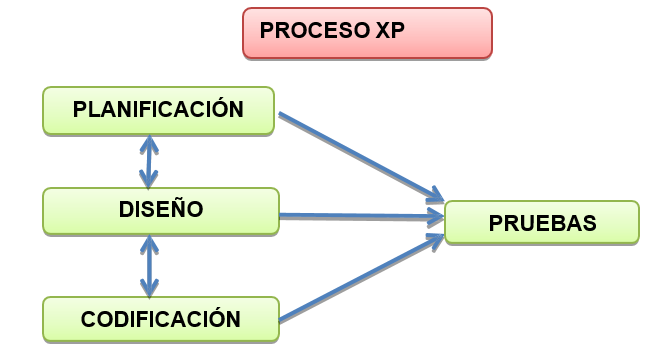
\includegraphics[width=.6\linewidth]{xp.png}
	\caption{Fases de XP ~\citep{VALLADAREZ2016}.}
	\label{fig:xp}
\end{figure}

\begin{itemize}
	\item \textbf{Planificaci�n}: La Metodolog�a \ac{XP} plantea la planificaci�n como un di�logo continuo entre las partes involucradas en el proyecto, incluyendo al cliente, a los programadores y a los coordinadores. El proyecto comienza recopilando las historias de usuarios, las que constituyen a los tradicionales casos de uso. Una vez obtenidas estas historias de usuarios, los programadores eval�an r�pidamente el tiempo de desarrollo de cada una, determinando as� el tiempo total de desarrollo del software.
	\item \textbf{Dise�o}: Especificaci�n de c�mo debe ser el dise�o final de la aplicaci�n, haciendo �nfasis en que un dise�o sencillo es m�s f�cil de implementar que uno complejo.
	\item \textbf{Codificaci�n}: Implementaci�n de los c�digos necesarios para satisfacer las historias de usuario.
	\item \textbf{Pruebas}: Una vez terminada la codificaci�n, se deben realizar las pruebas pertinentes a la misma.
\end{itemize}
\section{Historias de usuario}

\begin{userstory}
	\storyname{Crear resoluci�n}
	\storyuser{Specialist}
	\storyiter{1}
	\storypriority{ High }
	\storyrisk{ Low }
	\storypoints{0.8}
	\storyprogrammer{John Doe }
	\storydescription{\lipsum[1]}
	\storyobservation{\lipsum[1]}
\end{userstory}

\chapter{Propuesta de soluci�n}\label{c:chapter2}

\section*{Introducci�n del cap�tulo}
 El presente cap�tulo aborda las particularidades del sistema de gesti�n a desarrollar. Para registrar las principales caracter�sticas se hace uso de los \ac{rf} y \ac{rnf}. Estos describen las funcionalidades y atributos de calidad que debe poseer el software. En el cap�tulo \ref{c:chapter1}, se seleccion� la metodolog�a \ac{xp} como gu�a para el desarrollo del software; por lo tanto, se utilizan las \ac{hu} como herramienta para una descripci�n detallada de los \ac{rf} y la confecci�n del plan de iteraciones. Mediante el uso de este �ltimo, se proceder� a la estimaci�n del tiempo requerido para la culminaci�n del desarrollo del sistema y, con el uso de patrones de dise�o, se facilitar� la posterior descripci�n de las tarjetas \ac{crc}.
 
\section{Requisitos}\label{s:req}

\subsection{Requisitos funcionales}
En ingenier�a de software, los \ac{rf} definen un sistema o sus componentes; describen la funci�n que un software debe realizar, ya sean c�lculos, manipulaci�n de datos, procesos de negocios, entre otros.
Ayudan adem�s a capturar los comportamientos planificados para un sistema, este comportamiento puede ser expresado como una funci�n, servicio o tarea que un software debe realizar~\citep{requisitos}. A continuaci�n, se exponen los diferentes \ac{rf} planteados por el usuario:
\begin{RF}
\item Autenticar Usuario
\item Asignar rol a usuario
\\
\item Listar denuncias
\item Crear denuncia
\item Modificar denuncia
\item Eliminar denuncia
\item Buscar denuncia
%\item Exportar listado de denuncias
%\item Imprimir denuncia
%\item Imprimir listado de denuncias
\\
\item Listar resoluciones
\item Crear resoluci�n
\item Modificar resoluci�n
\item Eliminar resoluci�n
\item Exportar resoluci�n
\\
\item Listar comisiones
\item Crear comisi�n
\item Modificar comisi�n
\item Eliminar comisi�n
\item Buscar comisi�n
\\
\item Listar declaraciones
\item Crear declaraci�n
\item Modificar declaraci�n
\item Eliminar declaraci�n
\item Buscar declaraci�n
%\item Exportar declaraci�n
\\
\item Listar casos disciplinarios
\item Crear caso disciplinario
\item Modificar caso disciplinario
\item Buscar caso disciplinario
\\
\item Exportar Resoluci�n de caso
\item Exportar Expediente
\\
\item Listar roles
\item Crear rol
\item Modificar rol
\item Eliminar rol
\item Buscar rol
\end{RF}

\subsection{Requisitos no funcionales}
Los \ac{rnf}, como su nombre sugiere, son aquellos requerimientos que no se refieren directamente a las funciones espec�ficas que proporciona el sistema, sino a las propiedades emergentes de este como la fiabilidad, el tiempo de respuesta y la capacidad de almacenamiento. De forma alternativa definen las restricciones del sistema \citep{sommerville2011software}.\\
Los requisitos no funcionales de la aplicaci�n a desarrollar son:
\\
\noindent Usabilidad:
\begin{RNF}
\item El sistema debe ser una aplicaci�n web
\item La interfaz del sistema debe ser intuitiva y f�cil de usar
\end{RNF}
Hardware y software:
\begin{RNF}[resume]
\item El sistema operativo del servidor debe tener instalado la m�quina virtual de Java 
\item El ordenador donde se ejecute el servidor debe poseer como m�nimo 4GB de \ac{ram} y 10GB de almacenamiento.
\item El cliente del sistema se podr� ejecutar en los principales navegadores web: Google Chrome y navegadores basados en \gls{chromium}, Mozilla Firefox y Safari.
\end{RNF}
Seguridad:
\begin{RNF}[resume]
\item Solo se podr� acceder al sistema despu�s de estar autenticado con usuario y contrase�a v�lidos
\item Solo se podr�n usar las funcionalidades del sistema en dependencia de si el usuario autenticado posee los permisos requeridos para la misma
\end{RNF}
Dise�o e implementaci�n:
\begin{RNF}[resume]
\item Usar JavaScript como lenguaje de programaci�n del lado del cliente.
%\item Usar VueJS como marco de trabajo de desarrollo del lado del cliente.
\item Usar Java como lenguaje de programaci�n del lado del servidor.
\item Usar Spring Boot como \gls{framework} de desarrollo del lado del servidor.

\item Usar la metodolog�a de desarrollo de software \ac{xp}
\end{RNF}

\section{Historias de usuario}
\label{s:hu}
Las HU ser�n representadas mediante tablas divididas por las siguientes secciones:
\begin{description}

	\item [N�mero] Identificador entero incremental en el tiempo;
	\item [Nombre de historia de usuario] Identificador alfanum�rico para su uso
	      entre los desarrolladores y el cliente;
	\item[Usuario] Nombre y apellidos de la persona involucrada en el desarrollo de la \ac{hu};
	\item[Iteraci�n asignada] Identificador entero perteneciente a la iteraci�n en la cual se planea implementar la funcionalidad descrita en la \ac{hu};
	\item[Prioridad en negocio] Las historias de usuarios que describen funcionalidades imprescindibles en el desarrollo del sistema tienen prioridad alta; aquellas que debe tener el sistema, pero que no son necesarias para su funcionamiento, prioridad media; y auxiliares y que son independientes del sistema, prioridad baja.
	\item[Riesgo en desarrollo] Las historias de usuarios que, en caso de tener alg�n error de implementaci�n, puedan afectar la disponibilidad del sistema, tienen un riesgo de desarrollo alto; las \ac{hu} que puedan presentar errores y retrasan la entrega de la versi�n tienen riesgo de desarrollo medio; y las que puedan presentar errores, pero estos son tratados con facilidad y no afectan en desarrollo del proyecto, tienen riesgo de desarrollo bajo.

	\item[Puntos estimados] Tiempo estimado que tardar� el desarrollo de la \ac{hu};
	\item[Descripci�n] Breve descripci�n de \ac{hu};
	\item[Observaciones] Se�alamiento o advertencia del sistema;
	\item[Prototipo de interfaz] Prototipo de interfaz si aplica.
\end{description} \citep{Joskowicz2008}


Los t�tulos de las \ac{hu} generadas son:
\begin{enumerate}[label=HU \arabic*:]

	\item Autenticar Usuario (Prioridad Alta)

	\item Asignar rol a usuario (Prioridad Baja)

	\item Listar denuncias (Prioridad Alta)

	\item Crear una denuncia (Prioridad Alta)

	\item Modificar una denuncia (Prioridad Alta)

	\item Eliminar denuncias (Prioridad Alta)

	\item Buscar denuncias (Prioridad Baja)

	\item Archivar denuncias (Prioridad Alta)

	\item Listar resoluciones decanales (Prioridad Alta)

	\item Crear una resoluci�n decanal (Prioridad Alta)

	\item Modificar una resoluci�n decanal (Prioridad Alta)

	\item Eliminar resoluciones decanales (Prioridad Alta)

	\item Listar comisiones (Prioridad Alta)

	\item Crear comisiones (Prioridad Alta)

	\item Modificar una comisi�n (Prioridad Alta)

	\item Eliminar comisiones (Prioridad Alta)

	\item Buscar comisiones (Prioridad Baja)

	\item Listar declaraciones (Prioridad Alta)

	\item Crear declaraci�n (Prioridad Alta)

	\item Modificar declaraci�n (Prioridad Alta)

	\item Eliminar declaraciones (Prioridad Alta)

	\item Buscar declaraci�n (Prioridad Baja)

	\item Crear caso disciplinario (Prioridad Alta)

	\item Listar casos disciplinarios (Prioridad Alta)

	\item Modificar caso disciplinario (Prioridad Alta)

	\item Buscar caso disciplinario (Prioridad Baja)

	\item Cerrar caso disciplinario (Prioridad Media)

	\item Listar roles (Prioridad Baja)

	\item Crear roles (Prioridad Baja)

	\item Modificar roles (Prioridad Baja)

	\item Eliminar roles (Prioridad Baja)

	\item Buscar roles (Prioridad Baja)

	\item Exportar resoluciones decanales (Prioridad Baja)

	\item Exportar denuncias (Prioridad Baja)

	\item Exportar declaraciones (Prioridad Baja)

	\item Exportar conclusiones de casos (Prioridad Baja)

	\item Exportar resoluciones de casos (Prioridad Baja)

\end{enumerate}
A continuaci�n se presentan las \ac{hu} con mayor prioridad dentro del negocio, determinadas por el cliente e conjunto con el equipo de desarrollo. El resto se podr�n encontrar en la secci�n de ap�ndices \ref{app:hu}: Historias de Usuario.


\begin{userstory}
	\storyname{ Crear una denuncia }
	\storyuser{ Usuario }
	\storyiter{ 1 }
	\storypriority{ Alta }
	\storyrisk{ Medio }
	\storypoints{ 0.4 }
	\storyprogrammer{ \authorA }
	\storydescription{ Como Usuario quiero crear una denuncia para notificar r�pidamente al decano de una indisciplina cometida por uno o varios estudiantes }
	\storyobservation{ }
	\storyinterface{ 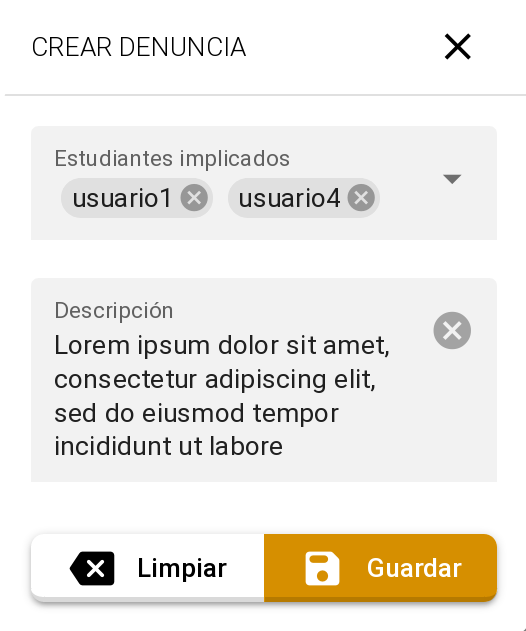
\includegraphics[width=0.5\textwidth]{images/prototypes/cdis-create-denuncia-capture.png} }
\end{userstory}

% Para crear un caso disciplinario basta con asignar una comisi�n a una denuncia pendiente:
% \begin{userstory}
% 	\storyname{ Crear caso disciplinario }
% 	\storyuser{ Decano }
% 	\storyiter{ 1 }
% 	\storypriority{ Alta }
% 	\storyrisk{ Medio }
% 	\storypoints{ 0.4 }
% 	\storyprogrammer{ \authorA }
% 	\storydescription{ Como Decano quiero crear caso disciplinario. }
% 	\storyobservation{ }
% 	\storyinterface{ 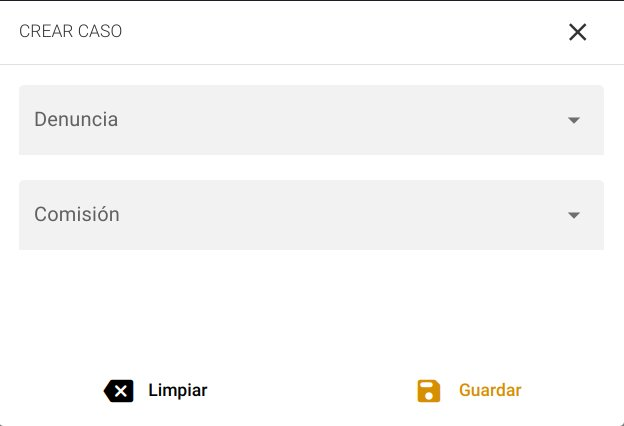
\includegraphics[width=0.5\textwidth]{images/prototypes/cdis-create-caso.png} }
% \end{userstory}
\section{Estimaci�n de esfuerzo por historia de usuario}
\begin {effortestimation}
\addentry[1]{ Listar denuncias }{0.2}
\addentry[1]{ Crear denuncia }{0.4}
\addentry[1]{ Modificar denuncia }{0.4}
\addentry[1]{ Eliminar denuncia }{0.4}

\addentry[1]{ Listar comisiones}{0.2}
\addentry[1]{ Crear comisi�n }{0.4}
\addentry[1]{ Modificar comisi�n }{0.4}
\addentry[1]{ Eliminar comisi�n }{0.4}

\addentry[1]{ Listar resoluciones }{0.2}
\addentry[1]{ Crear resoluci�n }{0.4}
\addentry[1]{ Modificar resoluci�n }{0.4}
\addentry[1]{ Eliminar resoluci�n }{0.4}

\addentry[2]{ Modificar roles de usuario }{0.2}
\addentry[2]{Listar rol}{0.2}
\addentry[2]{Crear rol}{0.4}
\addentry[2]{Modificar rol}{0.4}
\addentry[2]{Eliminar rol}{0.2}

\addentry[3]{ Exportar resoluci�n }{0.6}
\addentry[3]{ Exportar expediente }{0.6}
\end{effortestimation}
%\geniterationplan

\pagebreak
\section{Tarjetas CRC}\label{crc}


\begin{crccard}
   \crcclass{DenunciaController}
   \crcresp{
      \begin{itemize}
         \item crear: Crear una denuncia, la misma se archiva junto con el listado de acusados
         \item listar: Mostrar la denuncia requerida
         \item modificar: Modificar denuncia
         \item borrar: Eliminar denuncia
      \end{itemize}
   }
   \crccolab{
      UsuarioService\\
      DenunciaService\\
      Convertidor\\
      SesionDetails\\
      ValidatorDenuncia\\
      DenunciaUsuarioService\\
      ExpedienteService\\
      CasoUsuarioService\\
      JsonBorrarDenuncia\\
      JsonCrearDenuncia\\
      JsonModificarDenuncia\\
      E\_Denuncia\\
      Mensaje\\
      CasoUsuario\\
      Denuncia\\
      DenunciaUsuario\\
      Usuario\\
   }
\end{crccard}

\begin{crccard}
   \crcclass{ExpedienteController}
   \crcresp{
      \begin{itemize}
         \item listar: Mostrar todos los expedientes de cada estudiante denunciado
         \item modificar: Editar la informaci�n contenida en cada expediente
      \end{itemize}
   }
   \crccolab{
      JsonModificarExpediente\\
      E\_Expediente\\
      ValidatorExpediente\\
      Convertidor\\
      Mensaje\\
      Expediente\\
      ExpedientePK\\
      ExpedienteService\\
   }
\end{crccard}

\begin{crccard}
   \crcclass{ResolucionController}
   \crcresp{
      \begin{itemize}
         \item crear: Crear la resoluci�n con todas las comisiones disciplinarias que conlleva
         \item mostrar: Mostrar todas las resoluciones
         \item borrar: Eliminar una resoluci�n
         \item modificar: Editar una resoluci�n
      \end{itemize}
   }
   \crccolab{
      JsonBorrarResolucion\\
      E\_ExpedienteJsonCrearResolucion\\
      ComisionReducida\\
      JsonModificarResolucion\\
      E\_Resolucion\\
      ValidatorResolucion\\
      Convertidor\\
      Mensaje\\
      Comision\\
      ComisionUsuario\\
      ComisionUsuarioPK\\
      Resolucion\\
      ComisionService\\
      ComisionUsuarioService\\
      ResolucionService\\
      RolService\\
      UsuarioService\\
   }
\end{crccard}

\chapter{Validaci�n de la soluci�n}\label{c:chapter3}
\subsection*{Introducci�n del cap�tulo} El presente cap�tulo describe la etapa de validaci�n de la soluci�n. Para ello, se exponen las diferentes pruebas realizadas durante el desarrollo del sistema que llevan al lanzamiento de una soluci�n que resuelva la situaci�n problem�tica planteada.
\section{Pruebas}
Uno de los pilares de \ac{xp} es el proceso de pruebas. Esta metodolog�a de desarrollo anima a probar constantemente tanto como sea posible. Esto permite aumentar la calidad de los sistemas reduciendo el n�mero de errores no detectados y disminuyendo el tiempo transcurrido entre la aparici�n de un error y su detecci�n. Tambi�n permite aumentar la seguridad de evitar efectos colaterales no deseados a la hora de realizar  dise�ada por los programadores, y pruebas de aceptaci�n o pruebas funcionales destinadas a evaluar si al final de una iteraci�n se consigui� la funcionalidad requerida dise�adas por el cliente final \citep{gutierrez2006pruebas}.
Con el objetivo de comprobar que los sistemas desarrollados funcionan de acuerdo a las especificaciones descritas por el cliente, se realizaron diferentes pruebas teniendo en cuenta las caracter�sticas de los m�dulos.

\subsection{Pruebas unitarias}
\label{ss:unit-tests}
Las pruebas unitarias son una forma de comprobar que un fragmento de c�digo funciona correctamente.Son peque�os tests que validan el comportamiento de un objeto y la l�gica \citep{gutierrez2006pruebas}. \ac{xp} plantea la realizaci�n de pruebas unitarias continuas, frecuentemente repetidas y automatizadas, incluyendo pruebas de regresi�n, y aconseja escribir el c�digo de la prueba antes de la codificaci�n \citep{kniberg2007scrumyxp}.\\
Para la aplicaci�n de las pruebas unitarias a la soluci�n se emple� el framework JUnit el cual permite realizar la ejecuci�n de clases Java de manera controlada, para poder evaluar si el funcionamiento de cada uno de los m�todos de la clase se comporta como se espera. Es decir, en funci�n de alg�n valor de entrada se eval�a el valor de retorno esperado; si la clase cumple con la especificaci�n, entonces JUnit devolver� que el m�todo de la clase pas� exitosamente la prueba; en caso de que el valor esperado sea diferente al que regres� el m�todo durante la ejecuci�n, JUnit devolver� un fallo en el m�todo correspondiente.
\begin{figure}[htp]
	\centering
	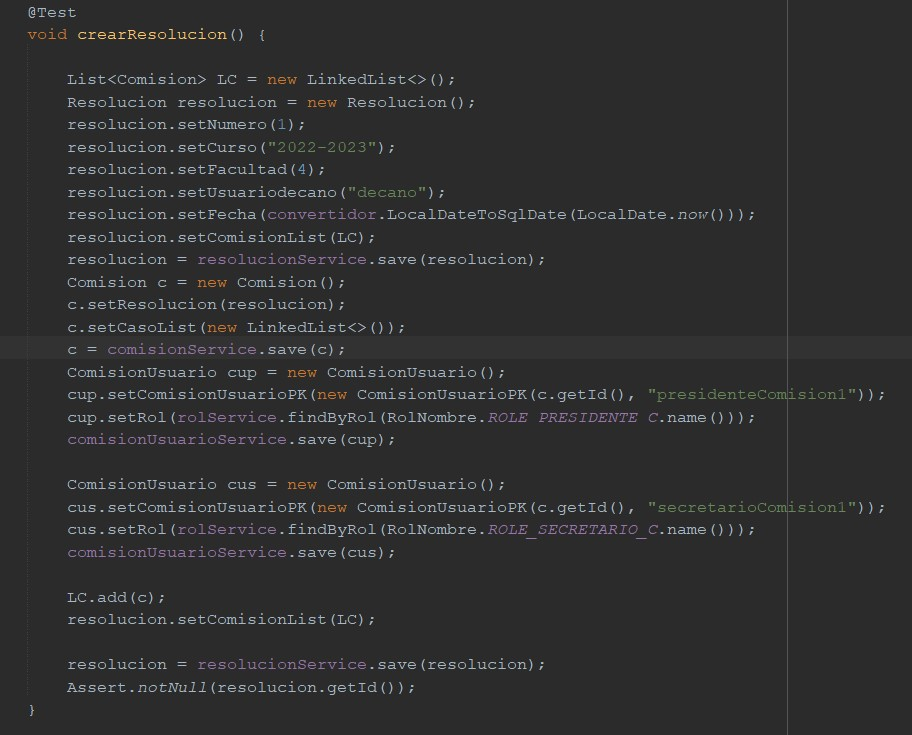
\includegraphics[width=0.8\textwidth]{images/test/PU1.jpg}
	\caption{Resultado de la ejecuci�n de pruebas unitarias en el c�digo fuente de CDIS. parte 1.}
	\label{fig:pu1}
\end{figure}
\begin{figure}[htp]
	\centering
	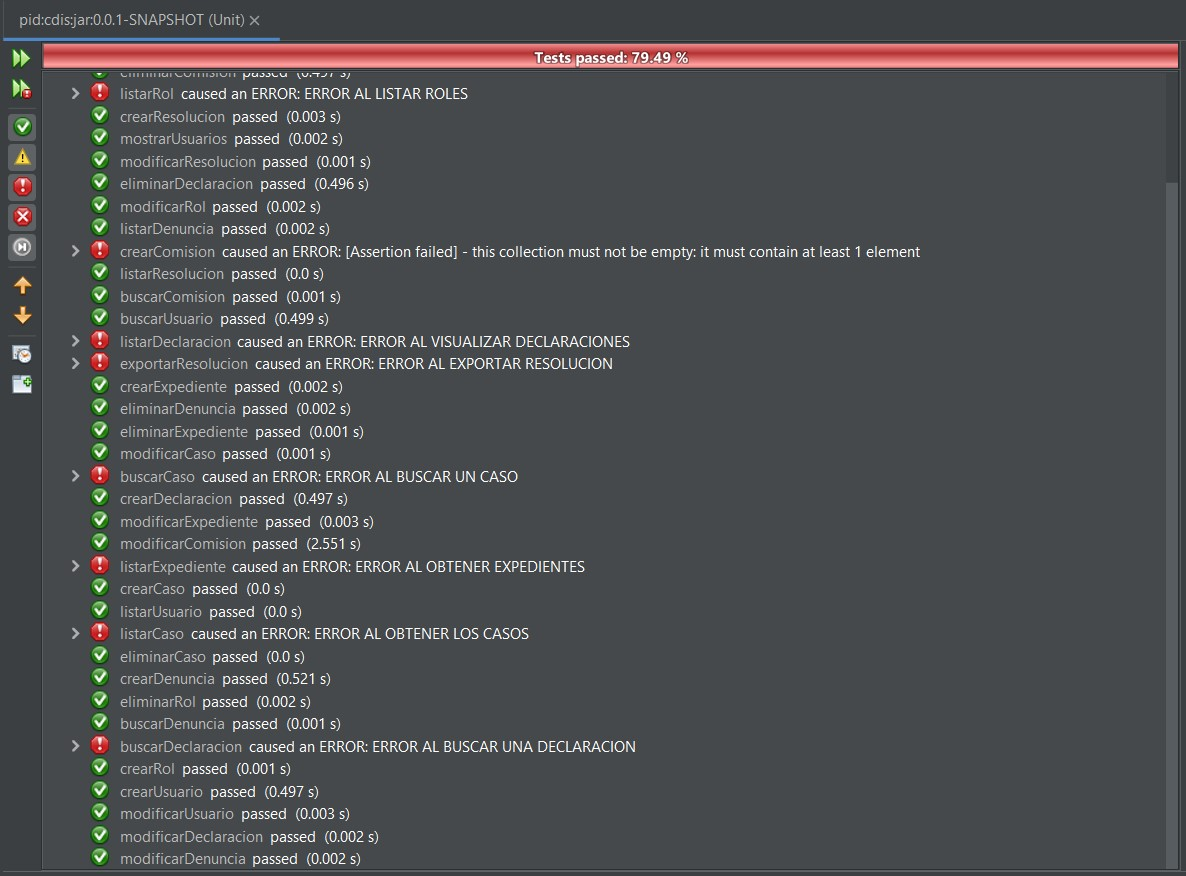
\includegraphics[width=0.8\textwidth]{images/test/PU2.jpg}
	\caption{Resultado de la ejecuci�n de pruebas unitarias en el c�digo fuente de CDIS. parte 2.}
\end{figure}

Se realizaron 39 pruebas unitarias al c�digo de las cuales 1 fue
fallida y se corrigi� exitosamente. A continuaci�n, se muestra el c�digo antes
de corregir el error detectado en la figura \ref{fig:pu1}:

\begin{figure}[htp]
	\centering
	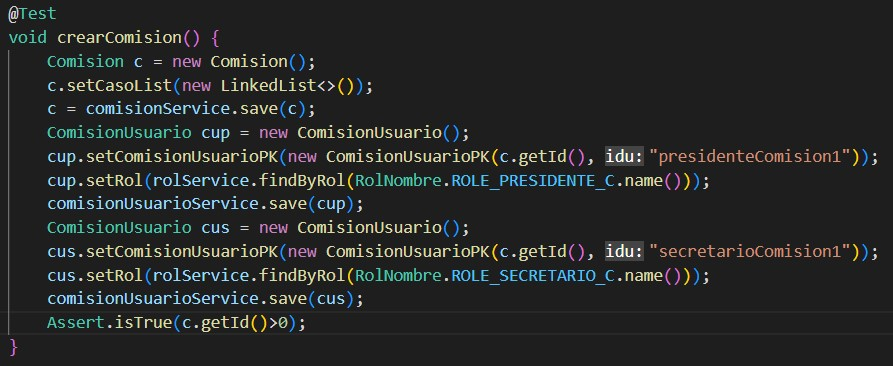
\includegraphics[width=0.8\textwidth]{images/test/before-error.jpg}
	\caption{M�todo crearComisi�n con error}
\end{figure}

Como se puede apreciar se est� intentando crear una comisi�n, pero por
alg�n motivo la l�gica del c�digo no fue bien planteada y terminamos
recibiendo una excepci�n causada a ra�z de que para crear una comisi�n
disciplinaria hace falta tambi�n asignarle una resoluci�n que la
contenga. La soluci�n a dicho problema se encuentra en la imagen
siguiente:
\clearpage
\begin{figure}[htp]
	\centering
	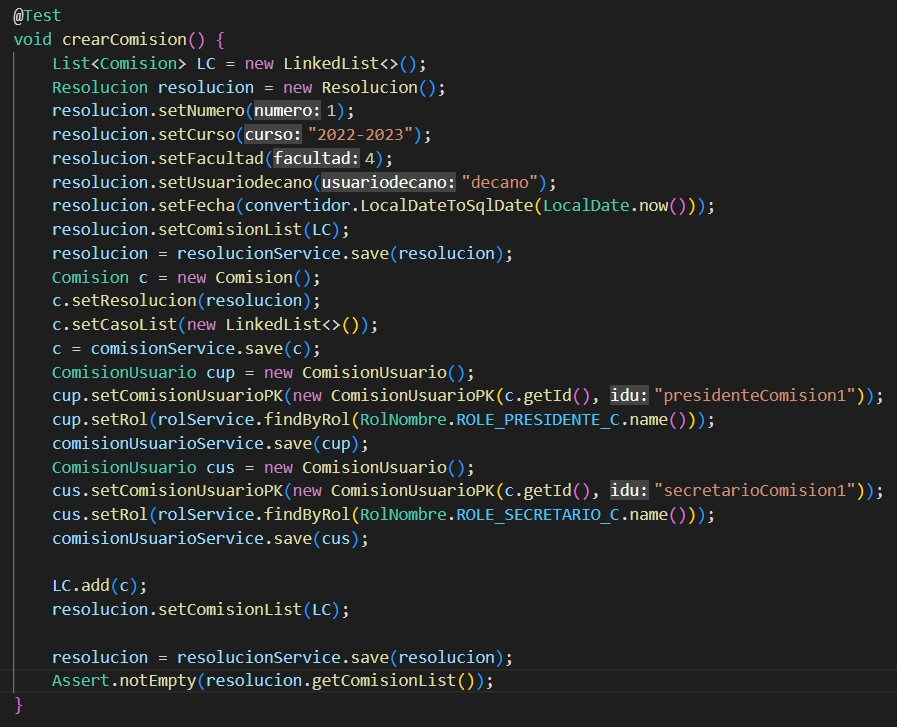
\includegraphics[width=0.8\textwidth]{images/test/after-error.jpg}
	\caption{M�todo crearComisi�n corregido}
\end{figure}

De esta forma garantizamos que una resoluci�n contiene la comisi�n que
estamos creando y esta se puede guardar con normalidad en la base de
datos.

Ahora se mostrar�n algunas im�genes de otras pruebas exitosas:

\begin{figure}[htp]
	\centering
	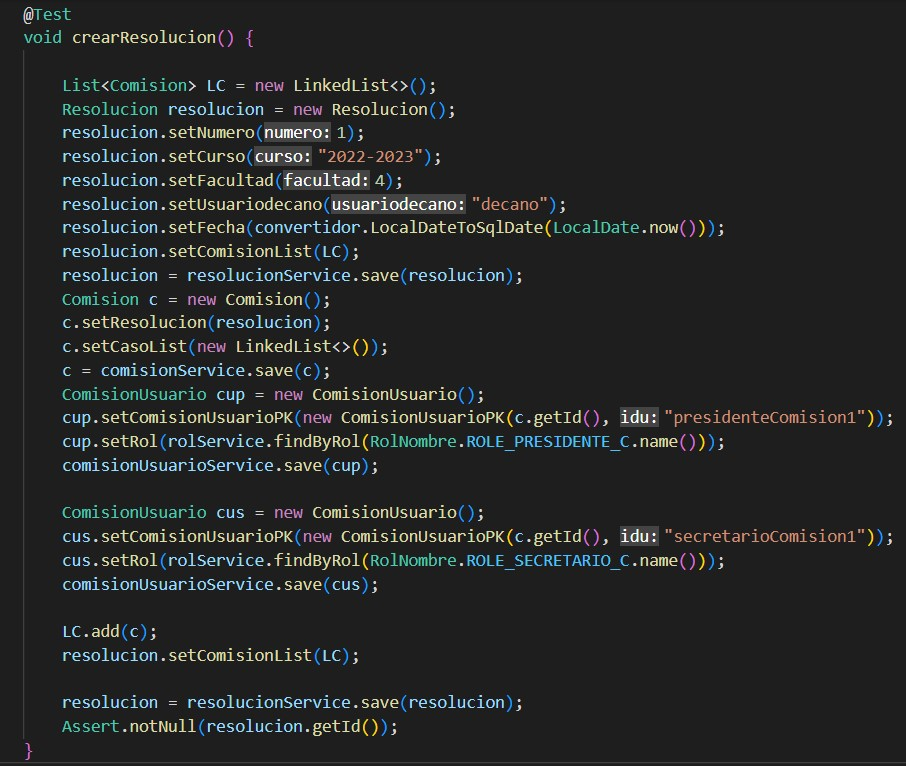
\includegraphics[width=0.8\textwidth]{images/test/E1.jpg}
	\caption{prueba para crearResoluci�n()}
\end{figure}

Se hace una prueba para crearResoluci�n(): Se comprueba que la
creaci�n de una resoluci�n sea exitosa despu�s de asignarle una comisi�n
disciplinaria

\begin{figure}[htp]
	\centering
	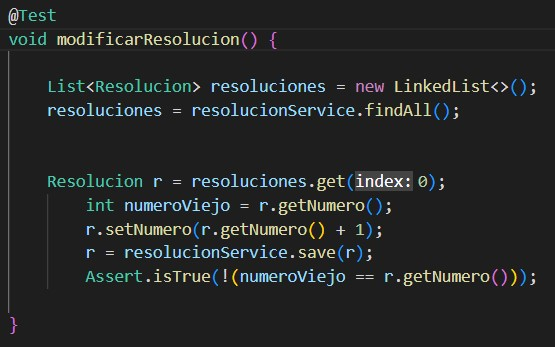
\includegraphics[width=0.8\textwidth]{images/test/E2.jpg}
	\caption{prueba para modificarResolucion()}
\end{figure}

Se hace una prueba para modificarResolucion(): Se actualiza la
informaci�n de una resoluci�n ya creada buscando fallas

\begin{figure}[htp]
	\centering
	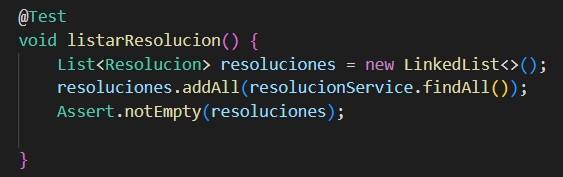
\includegraphics[width=0.8\textwidth]{images/test/E3.jpg}
	\caption{prueba para listarResolucion()}
\end{figure}

Se hace una prueba para listarResolucion(): Se llaman objetos
de la base de datos para guardarlos en un listado de objetos
de tipo: Resolucion

\begin{figure}[htp]
	\centering
	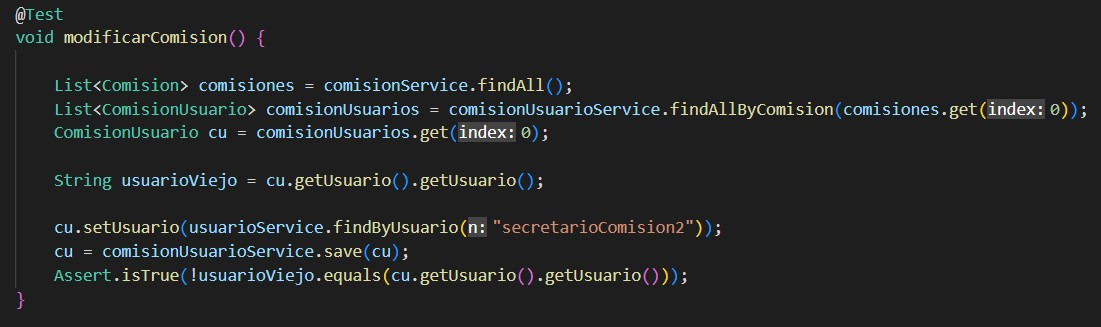
\includegraphics[width=0.8\textwidth]{images/test/E4.jpg}
	\caption{prueba para modificarComision()}
\end{figure}

Se hace una prueba para modificarComision(): Se actualiza la
informaci�n de una comisi�n seleccionada buscando fallas

\begin{figure}[htp]
	\centering
	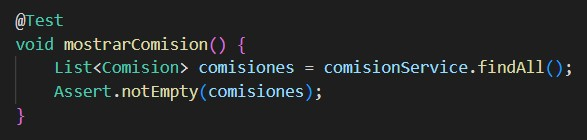
\includegraphics[width=0.8\textwidth]{images/test/E5.jpg}
	\caption{prueba para mostrarComisionl()}
\end{figure}

Se hace una prueba para mostrarComisionl(): Se llama a la
base de datos para obtener objetos de tipo: Comision

\begin{figure}[htp]
	\centering
	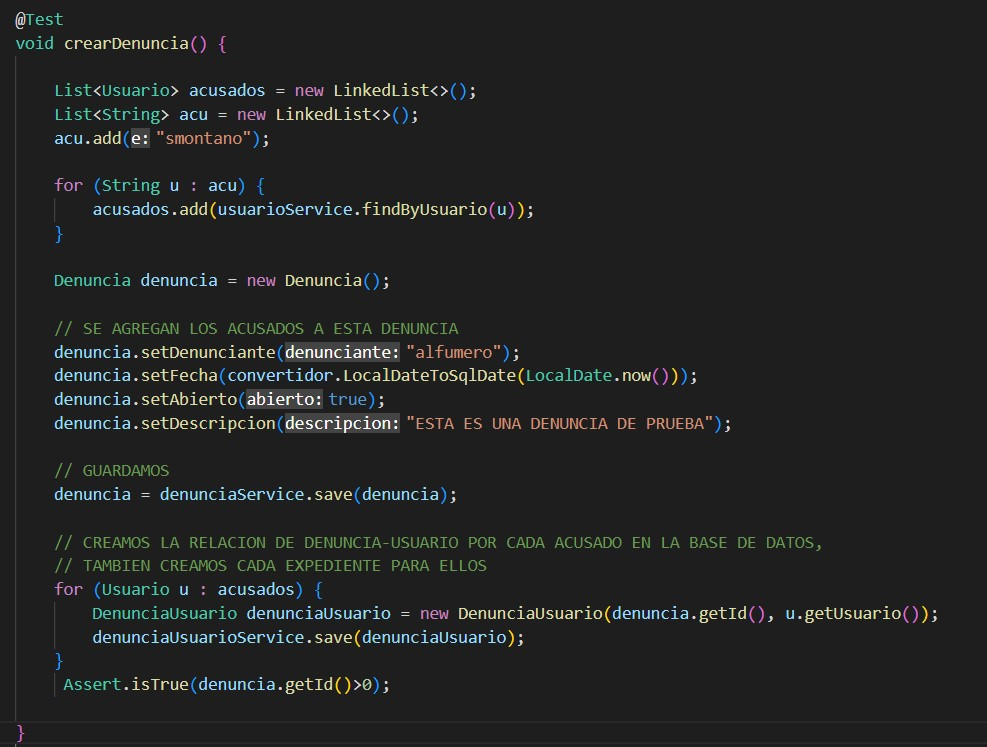
\includegraphics[width=0.8\textwidth]{images/test/E6.jpg}
	\caption{prueba para crearDenuncia()}
\end{figure}

Se hace una prueba para crearDenuncia(): Se crea una denuncia,
este es uno de los m�todos m�s importantes y base de la aplicaci�n

\begin{figure}[htp]
	\centering
	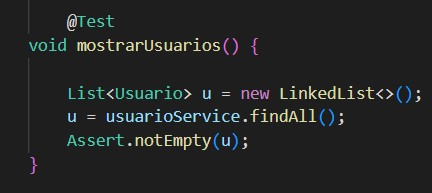
\includegraphics[width=0.8\textwidth]{images/test/E7.jpg}
	\caption{prueba para mostrarUsuarios()}
\end{figure}

Se hace una prueba para mostrarUsuarios(): Se comprueba que todos
los usuarios se muestren correctamente

\begin{figure}[htp]
	\centering
	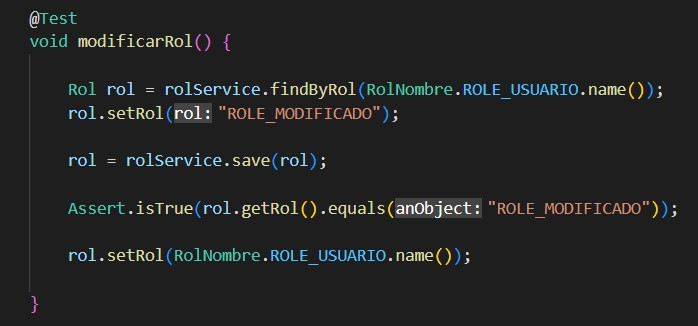
\includegraphics[width=0.8\textwidth]{images/test/E8.jpg}
	\caption{prueba para modificarRol()}
\end{figure}

se hace un test para modificarRol(): Se comprueba el correcto
funcionamiento en la actualizaci�n de los atributos del objeto de prueba de tipo: Rol

\clearpage

\subsection{Pruebas de aceptaci�n}
Las pruebas de aceptaci�n son definidas por el usuario del sistema y preparadas por el equipo de desarrollo, aunque la ejecuci�n y aprobaci�n final corresponden al usuario. Estas pruebas van dirigidas a comprobar que el sistema cumple los requisitos de funcionamiento esperado, recogidos en el cat�logo de requisitos y en los criterios de aceptaci�n del sistema de informaci�n, y conseguir as�? la aceptaci�n final del sistema por parte del usuario \citep{gutierrez2006pruebas}.
A continuaci�n se muestran algunas de las pruebas de aceptaci�n realizadas. 

\begin{acceptancetest}[t:hu1p1] % label in brackets
   \testcasecode{HU1\_P1}
   \testcasedescription{Prueba para la funcionalidad: Autenticar usuario. Prueba que s�lo se puede acceder a las funcionalidades del sistema si se ha realizado una autenticaci�n exitosa primero}
   \testcaseexeccond{El usuario no est� autenticado en el sistema.}
   \testcaseexecstep{
   \begin{enumerate}
   \item Se navega a la p�gina donde se encuentra el formulario de autenticaci�n.
   \item Se ingresan los credenciales correctos en el formulario de autenticaci�n.
   \item Se inicia la autenticaci�n a trav�z del bot�n de acci�n del formulario o la tecla Enter.
   \item Se recarga la p�gina.
   \end{enumerate}
   }
   \testcaseexpresult{El usuario queda autenticado en el sistema si se ingresan los credenciales correctos solamente. Se muestran los elementos de la interfaz que permiten acceder a las funcionalidades del sistema y la informaci�n del usuario autenticado justo despu�s de culminar el proceso de autenticaci�n.\\
      Evaluaci�n de la prueba: Satisfactoria}
   \testcasename{Autenticar usuario}
   \testcaseuserstory{1}
\end{acceptancetest}

\begin{acceptancetest}[t:hu1p2] % label in brackets
   \testcasecode{HU1\_P2}
   \testcasedescription{Prueba para la funcionalidad: Autenticar usuario. Prueba que el usuario puede cerrar una sesi�n iniciada.}
   \testcaseexeccond{El usuario est� autenticado en el sistema.}
   \testcaseexecstep{
   \begin{enumerate}
   \item Se inicia el cierre de sesi�n desde el men� del cliente.
   \item Se confirma la acci�n en un cuadro de di�logo.
   \item Se recarga la p�gina.
   \end{enumerate}
   }
   \testcaseexpresult{El usuario deja de estar autenticado en el sistema.\\
   Evaluaci�n de la prueba: Satisfactoria}
   \testcasename{Autenticar usuario}
   \testcaseuserstory{1}
\end{acceptancetest}
\section*{Conclusiones del cap�tulo}
Al finalizar el presente cap�tulo se arriba a las siguientes conclusiones parciales:

\begin{itemize}
    \item Definir una estrategia de pruebas contribuy� a un temprano descubrimiento de errores y no conformidades en la propuesta de soluci�n.
    \item Luego de cada cambio significativo en el sistema, se realizaron pruebas unitarias automatizadas a las principales funcionalidades, exigi�ndose un 100\% de efectividad para las mismas. Los resultados fueron buenos. Permitieron garantizar estabilidad durante el desarrollo y sentar las bases para las pruebas de sistema.
    \item Las pruebas de sistema permitieron validar la soluci�n, y verificar que se cumplieron los requisitos identificados por el cliente y el equipo de desarrollo para cada iteraci�n.
\end{itemize}
\conclusions
\suggestions
A partir de los resultados obtenidos se recomienda:
\begin{itemize}
    \item Implementar un m�dulo de an�lisis estad�stico.
    \item Incluir nuevas funcionalidades como manejo de apelaciones y comisiones mixtas.
\end{itemize}
\appendixes
\end{document}
